\chapter{Strumenti utilizzati}

\section{Front-end e back-end}
I termini front end (in sigla \textbf{ FE}) e back end (in sigla \textbf{BE}) denotano, rispettivamente, la parte visibile all'utente e con cui egli può interagire (interfaccia utente) e la parte che permette l'effettivo funzionamento di queste interazioni.
Il front end, è responsabile dell'acquisizione dei dati di ingresso e della loro elaborazione tali da renderli utilizzabili dal back end. \newline
Nella programmazione e sviluppo dei siti web viene definito front end la parte visibile da chiunque e raggiungibile all'indirizzo web del sito e viene definita back end la parte di amministrazione di un sito accessibile solo da amministratori del sito web. Front end e back end si utilizzano solamente quando il sito web è dinamico \cite{sito_frontback_end}. 


\section{Back End}

\subsection{Software}
Di seguito saranno introdotti vari strumenti software che hanno trovato ampio utilizzo per la realizzazione di questo progetto.
\subsubsection{Web Server}
Un server web (o web server) è un'applicazione software che, in esecuzione su un server, è in grado di gestire le richieste di trasferimento di pagine web di un client, tipicamente un web browser. La comunicazione tra server e client avviene tramite il protocollo \textbf{HTTP}, che utilizza la porta TCP 80 (o 8080), o eventualmente la versione sicura \textbf{HTTPS}, che utilizza invece la 443 \cite{sito_webserver}.
\newline
\newline
\newline
In questo progetto è stato utilizzato \textbf{Apache HTTP Server}.
Il Web Server Apache presenta un'architettura modulare, quindi ad ogni richiesta del client vengono svolte funzioni specifiche da ogni modulo di cui è composto, come unità indipendenti. Ciascun modulo si occupa di una funzionalità, ed il controllo è gestito dal core.
In linea continua il flusso dei dati reale
Tratteggiato il flusso dei dati astratto che forma la pipeline
Al di sopra del ciclo del core un demone esegue un ciclo di polling, attraverso il quale vengono interrogate continuamente le linee logiche da cui possono pervenire messaggi di richiesta.
Il core passa poi la richiesta ai vari moduli in modo sequenziale, usando i parametri di uscita di un modulo come parametri di accesso per il successivo, creando così l'illusione di una comunicazione orizzontale fra i moduli (Pipeline software) \cite{sito_apache}.
Le principali fasi di cui è composto il ciclo sono:
\begin{itemize}
\item \textbf{Translation}: traduce la richiesta del client
\textbf{Access Control}: controlla le richieste in base ai criteri di autorizzazione.
\item \textbf{MIME Type}: identifica il tipo di contenuto e decide quali moduli possono contribuire a servire la richiesta.
\item \textbf{Response}: invia la risposta al client e attiva eventuali procedure.
\item \textbf{Logging}: tiene traccia di tutto ciò che è stato fatto.
\end{itemize}

 \begin{figure}[h]
	\centering
	\caption {Architettura di Apache : In linea continua il flusso dei dati reale,
		tratteggiato il flusso dei dati astratto che forma la pipeline \cite{sito_apache}.}
	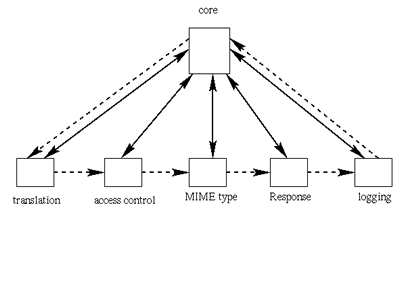
\includegraphics[scale = 0.8]{apache.png}
\end{figure}

\newpage

\subsubsection{Database Management System}
Un Database Management System, abbreviato in \textbf{DBMS} o Sistema di gestione di basi di dati, è un sistema software progettato per consentire la creazione, la manipolazione e l'interrogazione efficiente di database e ospitato su architettura hardware dedicata oppure su semplice computer \cite{sito_dbms}.\newline \newline
In questo progetto viene utilizzato \textbf{MySQL} che è un Relational database management system (\textbf{RDBMS}) composto da un client a riga di comando e un server. Entrambi i software sono disponibili sia per sistemi Unix e Unix-like sia per Windows.
\newline
MySQL è un software libero rilasciato a doppia licenza, compresa la GNU General Public License, ed è sviluppato per essere il più possibile conforme agli standard ANSI SQL e ODBC SQL \cite{sito_mysql_license}.
\newline
I sistemi e i linguaggi di programmazione che supportano MySQL sono molto numerosi: ODBC, Java, Mono, .NET, PHP, Python e molti altri.
\newline
In MySQL una tabella può essere di diversi tipi (o \textbf{storage engine}). Ogni tipo di tabella presenta proprietà e caratteristiche differenti (transazionale o meno, migliori prestazioni, diverse strategie di locking, funzioni particolari, ecc). 
Degna di nota è sicuramente il tipo di tabella \textbf{InnoDB} \cite{sito_innodb},
che mette a  disposizione le seguenti funzionalità:
\begin{itemize}
\item transazioni SQL con savepoint e transazioni XA;
\item lock a livello di record;
\item chiavi esterne (\textbf{Foreign Key});
\item buffer per gli indici, le chiavi, modifiche, cancellazioni;
\item compressione delle tabelle;
\item Il lock in InnoDB per quanto riguarda i comandi SELECT è di tipo non-locking. InnoDB offre delle ottime performance in termini di prestazioni e utilizzo della CPU.
\end{itemize}
Per quanto riguarda i limiti di questo tipo di tabella, si ha:
\begin{itemize}
\item Impossibilità creare più di 1000 colonne per tabella;
\item Su alcuni sistemi operativi le dimensioni del tablespace non possono superare i 2 GB;
\item La grandezza di tutti i file di log di InnoDB deve essere inferiore ai 4 GB;
\item	La grandezza minima di un tablespace è di 10 MB;
\item	Gli indici FULLTEXT sono stati introdotti nella versione 5.6 di MySQL e nella versione 10.0 di MariaDB, ma in alcune circostanze sono meno efficienti rispetto a quelli di \textbf{MyISAM} (storage engine predefinito in MySQL dalla sua introduzione (versione 3.23) fino alla versione 5.5).
\end{itemize}

\subsubsection{PhpMyAdmin}

PhpMyAdmin è un'applicazione web scritta in PHP, distribuita con licenza GPL, che consente di amministrare un database MySQL o MariaDB tramite un qualsiasi browser. 
\newline
PhpMyAdmin permette di creare un database da zero, creare le tabelle ed eseguire operazioni di ottimizzazione sulle stesse. Sono previste delle funzionalità per l'inserimento dei dati (popolazione del database), per le query, per il backup dei dati, e molto altro  \cite{sito_phpmyadmin}.
\newline


\subsubsection{XAMPP}
XAMPP è una piattaforma software multi-piattaforma e libera costituita da Apache HTTP Server, il gestore di database MariaDB (prima della versione 5.5.30 il gestore di database era MySQL)  e tutti gli strumenti necessari per utilizzare i linguaggi di programmazione PHP e Perl. Il nome è un acronimo dei software sopra citati (la X sta per x-platform, l'abbreviazione di cross-platform in lingua inglese ovvero multipiattaforma) \cite{sito_xampp}.
I componenti inclusi in questo pacchetto e utilizzati sono:
\begin{itemize}
\item il web server: \textbf{Apache} HTTP Server;
\item il database management system : \textbf{MariaDB} e SQLite; 
\item come linguaggio di programmazione: \textbf{PHP};
\item come modulo \textbf{PhpMyadmin}.
\end{itemize}


 \begin{figure}[h]
	\centering
	\caption{Pannello di XAMPP per Windows}
	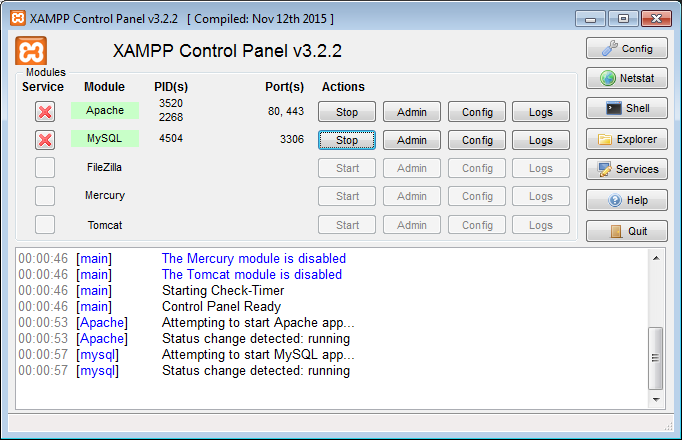
\includegraphics[scale = 0.8]{xampp.png}
\end{figure}

\newpage

\subsection{Linguaggi di Programmazione}
Verranno ora introdotti i linguaggi di programmazione utilizzati nella parte di \textbf{BE}.
\subsubsection{PHP}
Il PHP (acronimo ricorsivo di "PHP: Hypertext Preprocessor", preprocessore di ipertesti; originariamente acronimo di "Personal Home Page") è un linguaggio di scripting interpretato, originariamente concepito per la programmazione di pagine web dinamiche. L'interprete PHP è un software libero distribuito sotto la PHP License.
\newline
PHP è in grado di interfacciarsi a innumerevoli DBMS tra cui MySQL \cite{sito_php}. 

\subsubsection{SQL}
L' SQL (Structured Query Language) è un linguaggio standardizzato per database basati sul modello relazionale (RDBMS) progettato per: 
\begin{itemize}
\item creare e modificare schemi di database (DDL - Data Definition Language);
\item inserire, modificare e gestire dati memorizzati (DML - Data Manipulation Language);
\item interrogare i dati memorizzati (DQL - Data Query Language);
\item creare e gestire strumenti di controllo ed accesso ai dati (DCL - Data Control Language). 
\end{itemize}
SQL è un linguaggio per interrogare e gestire basi di dati mediante l'utilizzo di costrutti di programmazione denominati query. Con SQL si leggono, modificano, cancellano dati e si esercitano funzioni gestionali ed amministrative sul sistema dei database \cite{sito_sql}. 
Esso si divide in:
\begin{itemize}
\item Data Definition Language (DDL) - permette di creare e cancellare database o di modificarne la struttura;
\item Data Manipulation Language (DML) - permette di inserire, cancellare, modificare i dati;
\item Data Control Language (DCL) - permette di gestire gli utenti e i permessi;
\item Query language (QL) - permette di interrogare il database, cioè di leggere i dati;
\item Device Media Control Language (DMCL) - permette di controllare i supporti (memorie di massa) dove vengono memorizzati i dati.
\end{itemize}
\newpage

\section{Front End}
\subsection{Software}
\subsubsection{Web Browser}
Il web browser (o più semplicemente browser) è un'applicazione per il recupero, la presentazione e la navigazione di risorse sul web. Tali risorse (come pagine web, immagini o video) sono messe a disposizione sul World Wide Web (la rete globale che si appoggia su Internet), su una rete locale o sullo stesso computer dove il browser è in esecuzione. 
Nell'architettura di rete \textbf{client-server} di Internet il browser rappresenta dunque il client che fa richieste di risorse web ai vari web server e application server ospitanti rispettivamente siti web e applicazioni web. Esso rappresenta dunque il sistema software di interfacciamento dell'utente con la rete che rende la navigazione dell'utente tipicamente user-friendly, sebbene ai primordi della rete siano esistiti anche browser testuali da riga di comando su shell. I browser vengono principalmente utilizzati su personal computer, ma anche su altri dispositivi che consentono la navigazione in Internet, come i palmari e gli smartphone. Quelli più noti e diffusi sono Internet Explorer, Mozilla Firefox, Google Chrome, Safari, Opera e Internet Explorer \cite{sito_web_browser}.
\newline \newline
In questo progetto viene utilizzato \textbf{Mozilla Firefox} che è un web browser libero e multipiattaforma, mantenuto da Mozilla Foundation per la navigazione da desktop e il web browser \textbf{Safari} sviluppato dalla Apple Inc per i sistemi operativi iOS e macOS per la navigazione da mobile.

\subsubsection{Editor}
Viene utilizzato \textbf{Visual Studio Code} che è un editor di codice sorgente sviluppato da Microsoft per Windows, Linux e macOS. Esso include supporto per debugging, un controllo per Git integrato, Syntax highlighting, IntelliSense, Snippet e refactoring del codice. È anche personalizzabile: gli utenti possono cambiare il tema dell'editor, le scorciatoie da tastiera, e le preferenze. È un software libero, anche se la versione ufficiale è sotto una licenza proprietaria \cite{sito_visual_studio_code}.
\newline
Questo editor supporta la colorazione della sintassi per i linguaggi utilizzati nel progetto (\textbf{Syntax highlighting}) come è possibile vedere nella seguente immagine.

 \begin{figure}[H]
	\centering
	\caption{script php (config.php) per la connessione al database}
	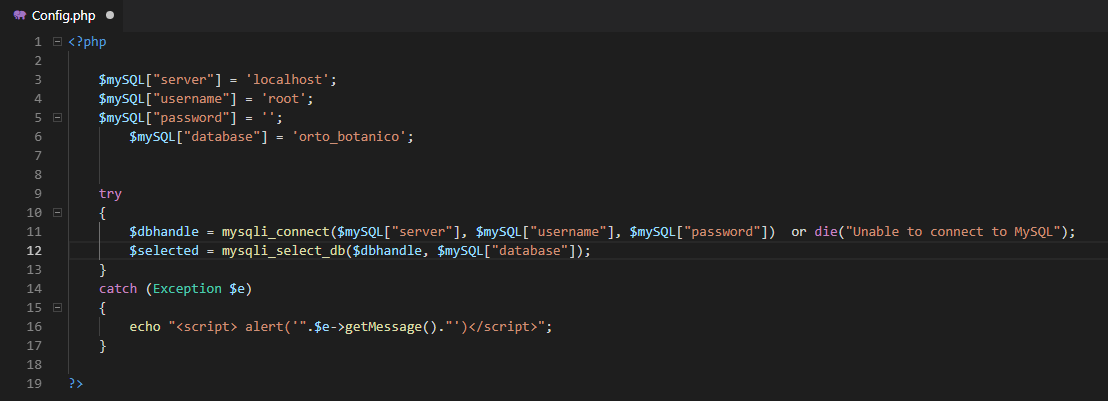
\includegraphics[width= 13cm]{visual_studio_code.png}
\end{figure}

\subsubsection{Leaflet}
Leaflet è una libreria JavaScript per sviluppare mappe geografiche interattive (WebGIS). Sviluppato dal 2010, supporta la maggior parte dei browser e degli standard HTML5 e CSS3. Permette di mostrare punti di interesse, linee o aree, o strutture dati come file GeoJSON, o livelli interattivi, su una mappa a tasselli \cite{sito_leaflet}. \newline
Punti di interesse (markers) e livelli (layers) possono essere aggiunti successivamente, in questo progetto viene fatta ampio uso di questa metodologia, aggiungendo e rimuovendo dinamicamente punti di interesse.
\begin{figure}[h]
	\centering
	\caption{immagine raffigurante dei punti di interesse: è possibile vedere il \textbf{polygon} che raffigura l'orto botanico \textit{Parco UNIVPM} con al centro un \textbf{circle} che cliccato apre il tooltip e i due \textbf{markers} che raffigurano i beacon (piante) nel parco.}
	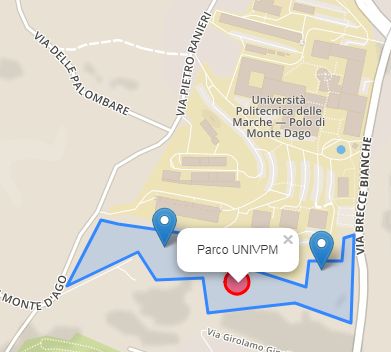
\includegraphics[width= 8cm]{leaflet.png}
\end{figure}

\subsubsection{W3C Geolocation API}
La W3C Geolocation API è una libreria del World Wide Web Consortium (W3C) per standardizzare un'interfaccia per recuperare le informazioni sulla posizione geografica di un dispositivo lato client. Le fonti più comuni di informazione sulla posizione dell'utente vengono stimate tramite :
\begin{itemize}
\item indirizzo IP;
\item Wi-Fi;
\item indirizzo MAC Bluetooth;
\item identificazione radio-frequenza (RFID);
\item posizione della connessione Wi-Fi;
\item Global Positioning System (GPS);
\item ID cella GSM / CDMA.
\end{itemize} 
La posizione dell'utente verrà restituita con una precisione determinata in base alla migliore fonte di informazione sulla posizione disponibile \cite{sito_geolocation_API}.

\subsubsection{WebRTC API}
WebRTC (Web Real-Time Communications) è una tecnologia che consente alle applicazioni Web e ai siti di acquisire e, a scelta, trasmettere contenuti audio e / o video, nonché di scambiare dati arbitrari tra browser senza richiedere un intermediario. L'insieme di standard che comprende WebRTC consente di condividere dati ed eseguire teleconferenze peer-to-peer, senza richiedere che l'utente installi plug-in o qualsiasi altro software di terze parti \cite{sito_WebRTC_API} \cite{sito_WebRTC_esempi}.

\newpage

\subsection{Linguaggi Utilizzati}
\subsubsection{HTML}
L'HyperText Markup Language è un \textbf{linguaggio di markup} che descrive le modalità di impaginazione o visualizzazione grafica (layout) del contenuto, testuale e non, di una pagina web attraverso tag di formattazione. Sebbene l'HTML supporti l'inserimento di script e oggetti esterni quali immagini o filmati, non è un linguaggio di programmazione: non prevedendo alcuna definizione di variabili, strutture dati, funzioni o strutture di controllo che possano realizzare programmi, il suo codice è in grado soltanto di strutturare e decorare dati testuali.
Quando un documento ipertestuale scritto in HTML è memorizzato in un file la sua estensione è tipicamente \textbf{.html} o \textbf{.htm}.
I documenti HTML vengono immagazzinati sui dischi rigidi di macchine elaboratrici (computer-server) costantemente collegate e connesse alla rete Internet. Su queste macchine è installato un software specifico (web server) che si occupa di produrre e inviare i documenti ai browser degli utenti che ne fanno richiesta usando il protocollo HTTP per il trasferimento dati \cite{sito_HTML}.

\subsubsection{CSS}

Il CSS (acronimo di Cascading Style Sheets, in italiano fogli di stile a cascata), è un linguaggio usato per definire la \textbf{formattazione} di documenti HTML, XHTML e XML. Le regole per comporre il CSS sono contenute in un insieme di direttive (Recommendations) emanate a partire dal 1996 dal W3C.
L'introduzione del CSS si è resa necessaria per separare i contenuti delle pagine HTML dalla loro formattazione e permettere una programmazione più chiara e facile da utilizzare, sia per gli autori delle pagine stesse sia per gli utenti, garantendo contemporaneamente anche il riutilizzo di codice ed una sua più facile manutenzione \cite{sito_CSS}.
Nessun browser attuale offre il supporto completo e corretto delle specifiche CSS. Tuttavia esistono browser che si avvicinano molto a questo risultato ed altri che invece ne sono molto lontani. La lista che segue è di motori di rendering perché a loro è assegnato il compito di formattare la pagina secondo le istruzioni CSS.

\subsubsection{CSS Framework CSS}
Un framework CSS è un software predisposto per consentire un web design più semplice e conforme agli standard utilizzando il linguaggio CSS. La maggior parte di questi framework contiene almeno una griglia. I framework più funzionali includono anche più funzionalità e funzioni aggiuntive basate su JavaScript e JQuery, ma sono principalmente orientati al design e non invadenti. \newline
Due esempi ampiamente utilizzati sono Bootstrap e \textbf{Materialize} (utilizzato in questo progetto) \cite{sito_framework_css}.

\subsubsection{Javascript}
JavaScript è un linguaggio di scripting orientato agli oggetti e agli eventi, comunemente utilizzato nella programmazione Web lato client per la creazione, in siti web e applicazioni web, di effetti dinamici interattivi tramite funzioni di script invocate da eventi innescati a loro volta in vari modi dall'utente sulla pagina web in uso (mouse, tastiera, caricamento della pagina ecc...).
\newline
Tali funzioni di script, utilizzati dunque nella logica di presentazione, possono essere opportunamente inserite in file HTML, in pagine JSP o in appositi file separati con estensione .js poi richiamati nella logica di business. 
\newline
Un uso principale del JavaScript in ambito Web è la scrittura di piccole funzioni integrate nelle pagine HTML che interagiscono con il DOM del browser per compiere determinate azioni non possibili con il solo HTML statico: controllare i valori nei campi di input, nascondere o visualizzare determinati elementi, ecc.
\newline
Sfortunatamente, gli standard DOM imposti dal W3C non sempre vengono rispettati dai vari browser: browser diversi (anche a seconda del loro motore di rendering) espongono diversi oggetti o metodi allo script (Internet Explorer è solito aderire agli standard con piccole modifiche, e tratta ad esempio l'oggetto event come globale), ed è quindi spesso necessario implementare controlli aggiuntivi ad una funzione JavaScript, per garantirne la compatibilità con ciascun browser \cite{sito_Js}.

\subsubsection{JQuery}
JQuery è una libreria JavaScript per applicazioni web. Nasce con l'obiettivo di semplificare la selezione, la manipolazione, la gestione degli eventi e l'animazione di elementi DOM in pagine HTML, nonché implementare funzionalità \textbf{AJAX} \cite{sito_JQuery}.

\subsubsection{AJAX}
AJAX, acronimo di Asynchronous JavaScript and XML, è una tecnica di sviluppo software per la realizzazione di applicazioni web interattive (Rich Internet Application). Lo sviluppo di applicazioni HTML con AJAX si basa su uno scambio di dati in background fra web browser e server, che consente l'aggiornamento dinamico di una pagina web senza esplicito ricaricamento da parte dell'utente.
\newline
La tecnica AJAX utilizza una combinazione di:
\begin{itemize}
	\item HTML (o XHTML) e CSS per il markup e lo stile;
	\item DOM (Document Object Model) manipolato attraverso un linguaggio ECMAScript come JavaScript o JScript per mostrare le informazioni ed interagirvi;
	\item l'oggetto XMLHttpRequest per l'interscambio asincrono dei dati tra il browser dell'utente e il web server. In alcuni framework AJAX e in certe situazioni, può essere usato un oggetto Iframe invece di XMLHttpRequest per scambiare i dati con il server e, in altre implementazioni, tag <script> aggiunti dinamicamente (JSON);
	\item in genere viene usato XML come formato di scambio dei dati, anche se di fatto qualunque formato può essere utilizzato, incluso testo semplice, HTML preformattato, JSON e perfino EBML. Questi file sono solitamente generati dinamicamente da script lato server. 
\end{itemize}
AJAX non è una tecnologia individuale, quanto piuttosto un gruppo di tecnologie utilizzate insieme.
\newline
Le applicazioni web che usano AJAX richiedono browser che supportano le tecnologie necessarie (quelle dell'elenco sopra). \newline Questi browser includono: Firefox, Opera, Konqueror, Safari, Internet Explorer e Chrome. Tuttavia, per specifica, \textit{Opera non supporta la formattazione degli oggetti XSL} \cite{sito_Ajax}.
